\chapter{Conclusion and Outlook} \label{ch:cando}

\section{8 TeV Inclusive Jet Results from CMS and ATLAS}

CMS\cite{CMS:2013kda} and ATLAS\cite{Aaboud:2017dvo} both reported the double differential cross section for inclusive jets at 8 TeV.  

\begin{figure}[h]
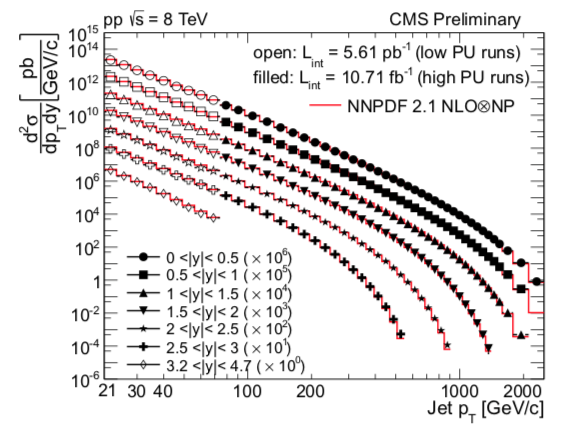
\includegraphics[width=10.0cm]{CMS8TeVJet}
\centering
\caption{8 TeV CMS inclusive jet cross sections with radii of R = 0.7 and binned by jet rapidity compared to NLO calculations with non-pertubative corrections\cite{CMS:2013kda}.}
\label{fig:CMS8TeVRescale}
\end{figure}

\begin{figure}[h]
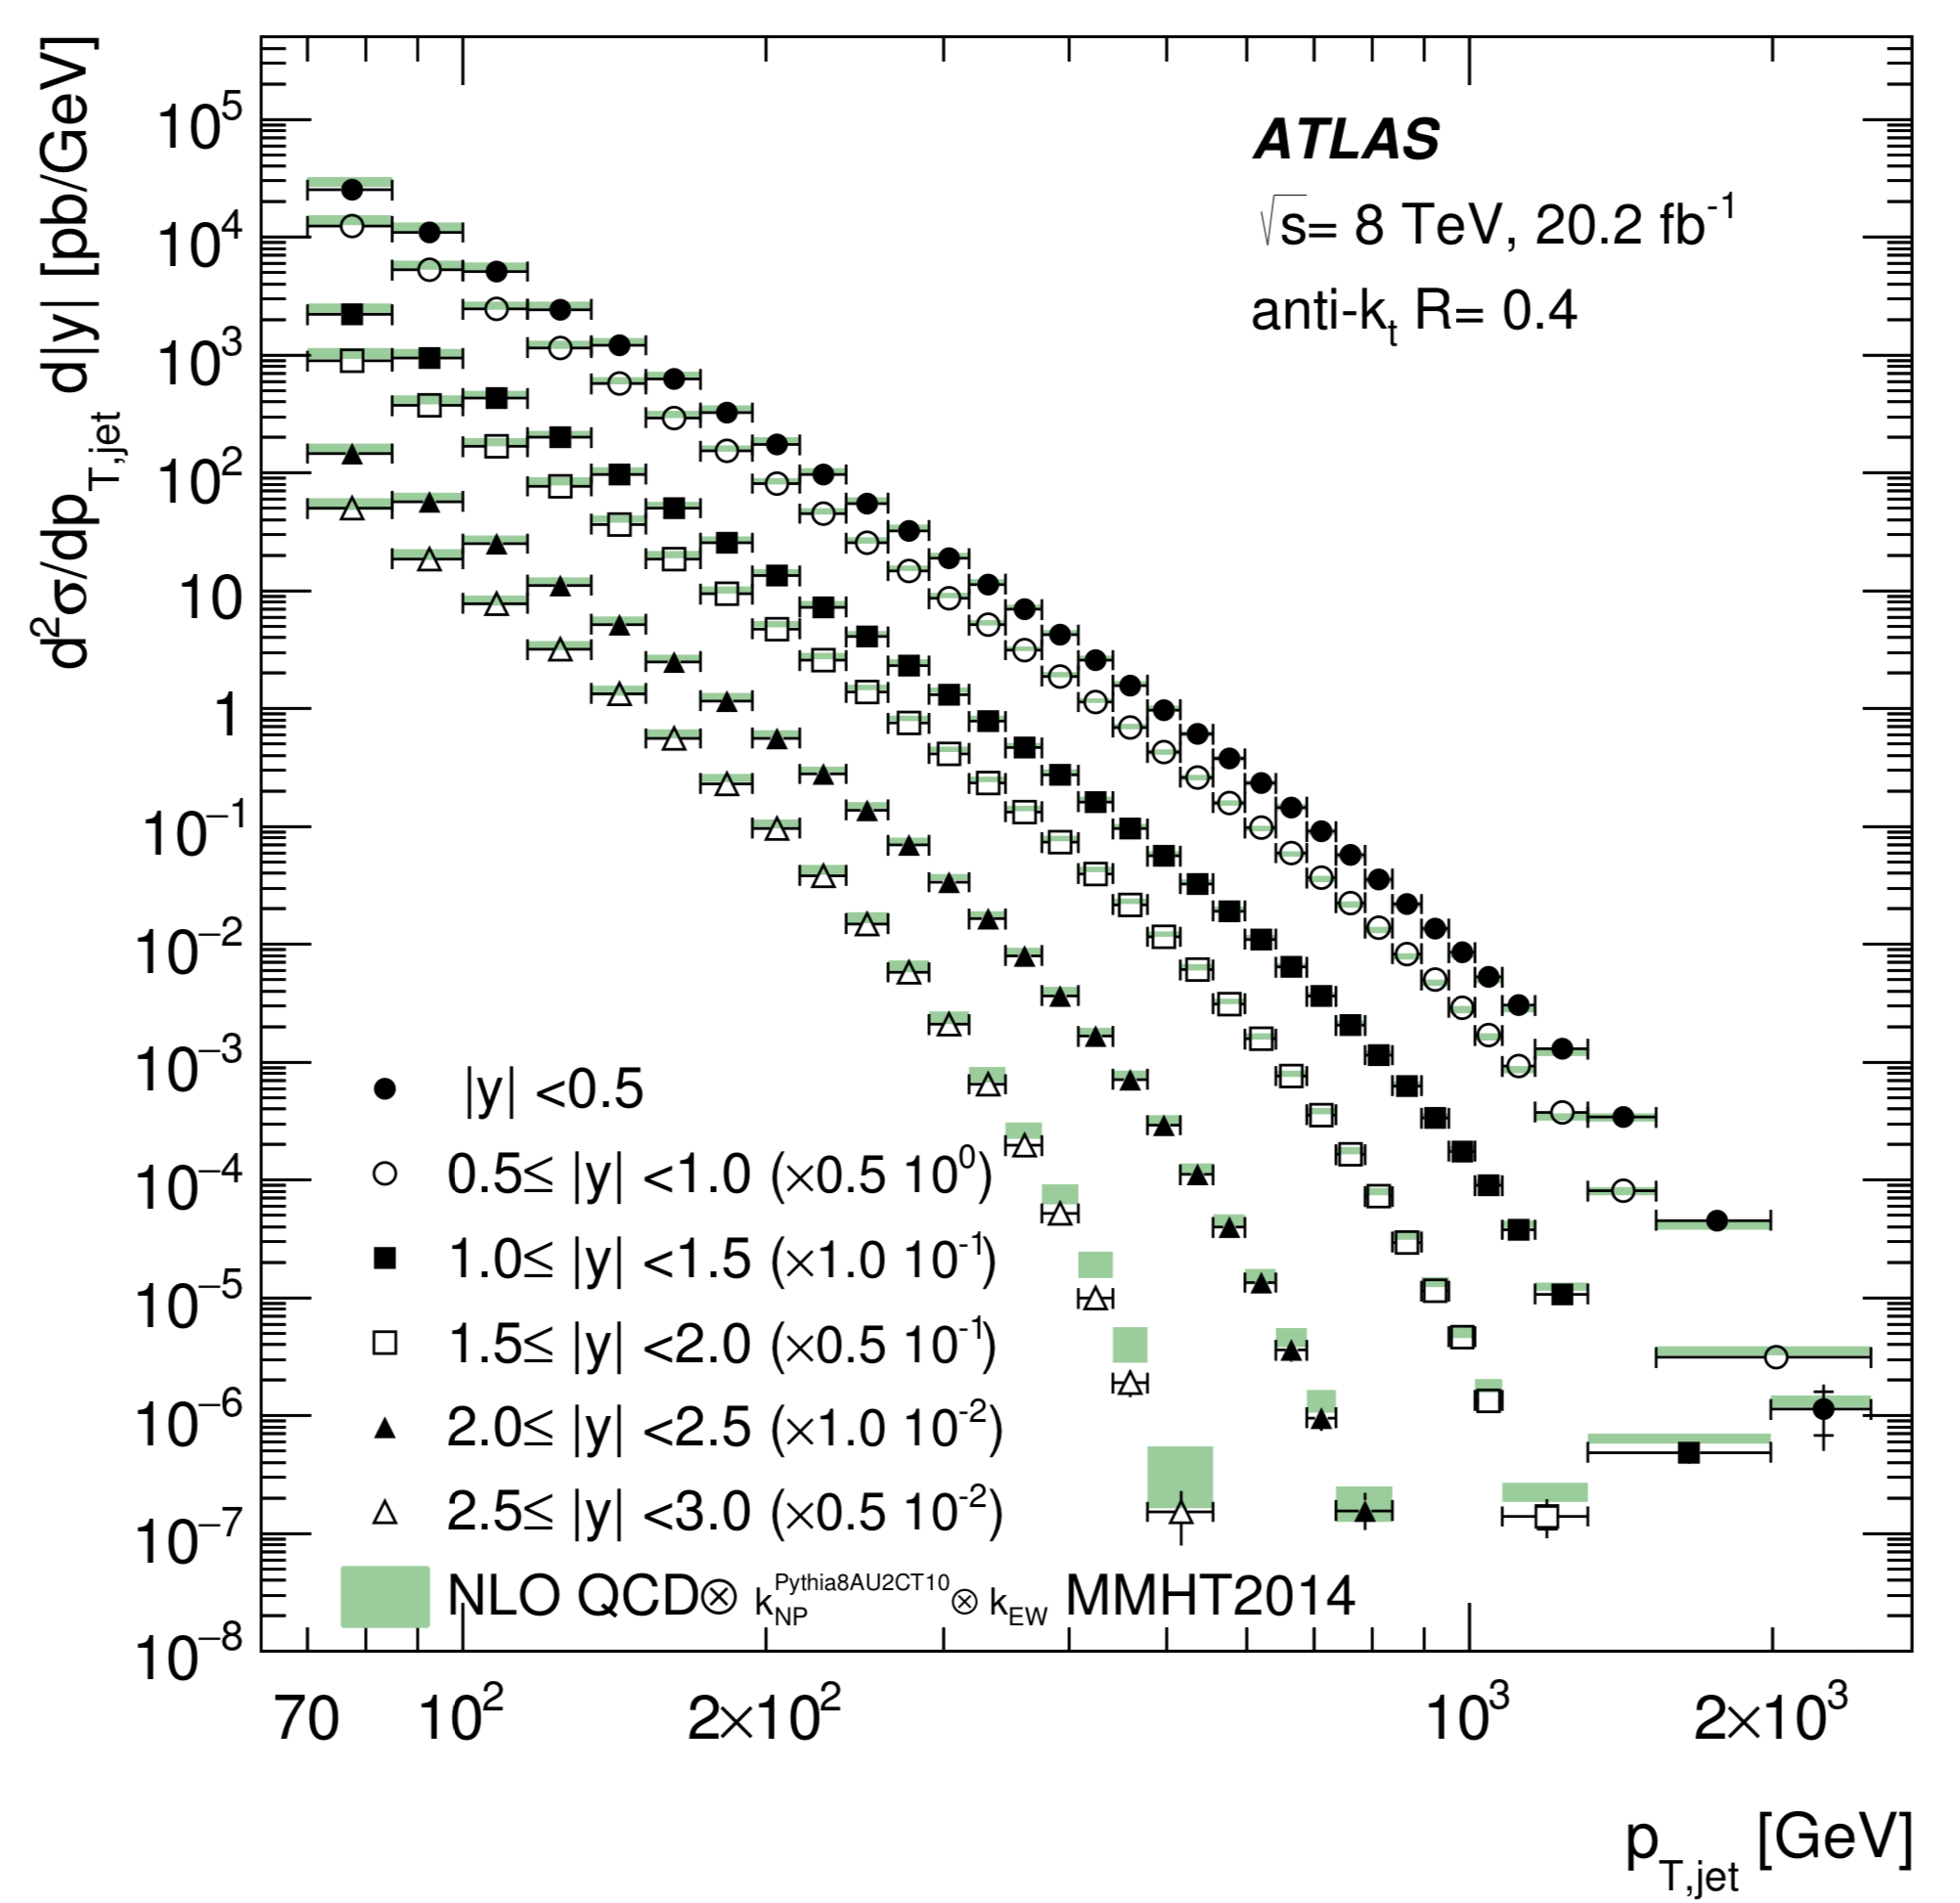
\includegraphics[width=10.0cm]{ATLAS8TeVJet}
\centering
\caption{R = 0.4 inclusive jet cross section at 8 TeV from ATLAS in binned by jet rapidity compared to NLO QCD predictions\cite{Aaboud:2017dvo}.}
\label{fig:ATLAS8TeV}
\end{figure}

\begin{figure}[h]
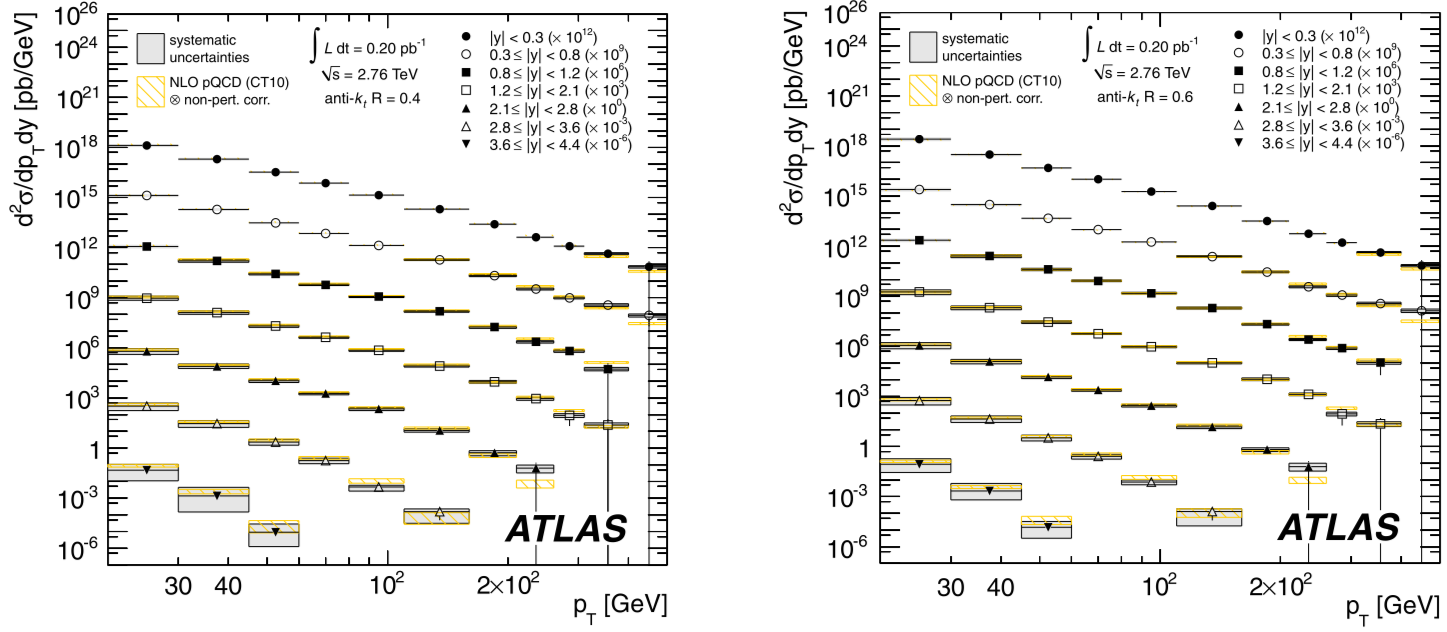
\includegraphics[width=14.0cm]{ATLAS8TeVJetRecaled}
\centering
\caption{The 8 TeV ATLAS jet cross sections rescaled to better show comparissons with NLO and non-pertubative calculations at low $p_{T}$\cite{Aaboud:2017dvo}.}
\label{fig:ATLAS8TeVRescale}
\end{figure}

